\documentclass{article}
\usepackage{pgfplots}
\usepackage{hyperref}
\usepackage{amsmath}
\usepackage{amsfonts}
\usepackage{amssymb}
\usepackage{graphicx}
\usepackage{listings}
\usepackage{float}
\usepackage{tikz}
\usepackage{circuitikz}
\usepackage{color}
\renewcommand{\labelenumi}{\arabic{enumi}.}
\renewcommand{\labelenumii}{\arabic{enumi}.\arabic{enumii}}
\usepackage{enumitem}
\definecolor{mauve}{RGB}{204,153,255}
\definecolor{mylilas}{RGB}{200,162,200}
\definecolor{pageno}{gray}{0.30}

\title{Physics Problem Set 2} \date{14-09-2015} \author{Hrishi Olickel}

\begin{document}
 \pagenumbering{gobble}
 \maketitle
 \newpage
 \tableofcontents
 \pagenumbering{arabic}
 \newpage
 
 \graphicspath{ {/} }
\lstdefinestyle{MATLAB}{ % 
    %basicstyle=\color{red},
    language = Matlab,
    breaklines=true,%
    morekeywords={matlab2tikz},
    frame=single,
    keywordstyle=\color{blue},%
    morekeywords=[2]{1}, keywordstyle=[2]{\color{black}},
    identifierstyle=\color{black},%
    stringstyle=\color{mylilas},
    commentstyle=\color{green},%
    showstringspaces=false,%without this there will be a symbol in the places where there is a space
    numbers=left,%
    numberstyle={\tiny \color{black}},% size of the numbers
    numbersep=9pt, % this defines how far the numbers are from the text
    emph=[1]{for,end,break},emphstyle=[1]\color{red}, %some words to emphasise
    %emph=[2]{word1,word2}, emphstyle=[2]{style},    
} 

\lstset{style=MATLAB}

\section{Answers}

\begin{enumerate}
\item Part 1
\begin{enumerate}[label*=\arabic*.]
 \item Since the item is a conductor, it has free flowing charges on the inside. If the electric field anywhere inside the surface of the material was not zero, these free charges would be animation and would violate our condition of resting charges.
 	Hence, we start with the assumption that the charge at any point inside a conductor must be zero. This is known to be true, since a non-zero value at point inside the conductor would cause flux within the conductor itself. Considering the smallest possible example of a conductor, a point with a boundary surrounding it, we find that the charge must be equally distributed within the boundary. Increasing the size, we can find inductively that the charge on any conductor at rest must reside on the surface.
 \item 
 	  A Faraday Cage can be considered a hollow conductor. When an external electric field is applied to the outside of the cage, the free flowing charges will re-arrange to cancel the field on the inside of the cage. Thus, any objects placed inside a Faraday cage are protected from the electric field outside the cage.
	  
 \item This Equation is given:
 \[ \Phi = E \times A \]
 From the symmetry of an infinite sheet, we can surmise that the electric field is independent of the distance.
 Accounting for both sides,
 \[ \Phi = E \times A \times 2 \]
 \[ \Phi = \sigma \times A / \epsilon 0 \]
\[ E = \frac{\sigma}{2 \times \epsilon 0} \]

\item 
	\[ mass = 8.20 \times 10^{-19} kg \]
	\[ q = 6.50 \times 10^9 C \]
	\[Surface Charge Density = 5.90 \times 10^{-8} C/m^2 \]
	\[ E = 5.90 \times \frac{10^{-8}}{2 \times \epsilon 0} = 3330 (3sf) \]
	
	Work done moving the charge from 0.4m to 0.1m will be 
	\[ W = E \times q \times ds = 6.497 \times 10^12 J \]
	
	Using $KE = \frac{1}{2}mv^2$, 
	\[ E = 0.5 \times m \times v^2 \]
	
	\[ \therefore v = 1.26 \times 10^{15} ms^{-1} \]
	
\item If the electric field of a point charge were proportional to $\frac{1}{r^3}$, it would be relational to three dimensional values, such as the size of the Gaussian surface. Gauss's Law would then be invalid because it clearly states that flux is only dependent on the charge it encloses, and not the size of the Gaussian Surface.

\item 

 \end{enumerate}
 \item Part 2
 \begin{enumerate}[label*=\arabic*.]
 	\item First, let us find the total resistance of the two resistors (3K and 1K) in parallel:
	\[ R_{combined} = \frac{1}{\frac{1}{A}+\frac{1}{B}} = \frac{1}{\frac{1}{3}+\frac{1}{1}} = \frac{3}{4}\]
	Now, we know that $I = \frac{V}{R}$. from this we can find the total current in the circuit:
	\[ R_{circuit} = 1 + \frac{3}{4} = \frac{7}{4}\]
	\[ I_{circuit} = \frac{5V}{\frac{7}{4}} = \frac{20}{7} \]
	Now it becomes simple to calculate the current flowing through the 3K resistor using Kirchoff's Laws:
	\begin{equation}
	I_A = \frac{3}{4} \times \frac{20}{7} = \frac{15}{7} = 2.14\,A
	\end{equation}
	
	\item The combined resistance of the $R_1$ $R_L$ segment can be summarised as $R_{comb}$ where:
	\[R_{comb} = \frac{R_L \times R_1}{R_L + R_1}\]
	From this, we can see that as $R_L \to \infty$, $R_{comb} \to R_1$ and as $R_L \to 0$, $R_{comb} \to 0$. Now we know the relationship between the $R_{comb}$ and $R_2$: 
	\begin{equation}
	V_{out} = V_{in} \times \frac{R_{comb}}{R_{comb}+R_2}
	\end{equation}
	From this, we can see that as $R_L \to \infty$,
	\[V_{out} \to V_{in} \times \frac{R_1}{R_1+R_2} \]
	
	\item Here, we can simply substitute the intermediate expressions for $R_{comb}$ and $V_{out}$  to find the expression:
	\[V_{out} = V_{in} \times \frac{\frac{R_L \times R_1}{R_L + R_1}}{\frac{R_L \times R_1}{R_L + R_1}+R_2} \]
	\[\therefore V_{out} = \frac{V_{in}}{R_2 \times (R_L+R_1)} \]
	
	\item For this rather large question, let us consider the resistances of the following sections:
	\[R_{56} = R_5+R_6 = 12 \Omega \]
	\[R_{456} = R_4 || R_{56} = \frac{16 \times 12}{16+12} = \frac{54}{7} \Omega \]
	\[R_{2456} = R_2 + R_{456} = \frac{68}{7} \Omega \]
	\[R_{32456} = R_3 || R_{2456} = \frac{204}{71} \Omega \]
	\[R_{132456} = R_1 + R_{32456} = \frac{346}{71} \Omega \]
	
	Using the final resistance, we can find the following equation for $I_{total}$:
	\[I_{total} = V_{total} \times \frac{346}{71} \]
	\[I_{34256} = V_{total} \times \frac{346}{71} \]
	\[I_{4256} =  V_{total} \times \frac{346}{71} \times \frac{R_{2456}}{R_{2456}+R_3} \]
	\[I_{56} = V_{total} \times \frac{346}{71} \times \frac{R_{2456}}{R_{2456}+R_3} \times \frac{R_5+R_6}{R_5+R_6+R_4} = 1.40 A \]
	\[\ V_{total} \times 0.1346 = 1.40 A \]
	\[ \therefore  V_{total} = 10.4 V \]
	
	
	
 \end{enumerate}
 \item Part 3
 \begin{enumerate}[label*=\arabic*.]
 
 	\item For the case of zero viscosity, when we assume $k=0$, we get the following:
	
	\[ F_{tot} = mg \]
	\[ a = g \]
	
	\begin{equation}
	\therefore a \leqslant g
	\end{equation}
	
	For the case of steady state motion we can assume terminal velocity and hence
	\[ \ddot{x} = 0 \]
	\[ \dot{x}^2 = g \]
	\[ \dot{x} = \sqrt{g} \]
	
	\begin{equation}
	\therefore \dot{x} \leqslant \sqrt{g}
	\end{equation}
	
	From these two derived limits we can conceive of the following sketches for v(t):
	
	\begin{tikzpicture}
	
		\begin{axis}[
			ticks=none,
			xlabel=$t$,
			ylabel={$v(t)$},
			xmin=0,
			ymax=10,
			xmax=100
			]
			\addplot [domain=0:100,samples=1000]{ln(x)+2};
			\addplot[domain=0:100,samples=1000,dashed] {7}node[above,pos=0]{$v=\sqrt{g}$};
		\end{axis}
	\end{tikzpicture}
	
	Similarly, x(t) becomes:
	
	\begin{tikzpicture}
		\begin{axis}[
		ticks=none,
		xlabel=$t$,
		ylabel={$x(t)$},
		xmin=0,
		ymax=5,
		xmax=4]
		\addplot[domain=0:1]{x^2};
		\addplot[domain=1:4]{2*x-1};
		\addplot[domain=0:4,dashed]{2*x-1}node[above,pos=0]{$\dot{x}=\sqrt{g}$};
		\end{axis}
	\end{tikzpicture}
	
\item From the sketches so far, the plot for the phase space is likely to have a steady state line running along $v=\sqrt{g}$, and any point above or below is likely to follow a trajectory that converges toward the steady state line. For example, when x=0 and v=0, x and v will steadily increase until $v=\sqrt{g}$, at which point x will continue increasing and v still remain constant.
When $x=0$, and $v>100$ or a value above $\sqrt{g}$, x will continue increasing and v will decrease until $v=\sqrt{g}$, at which point the steady state occurs.

\item The following code was used: 
	\begin{lstlisting}
	    function xdot = f(x,t)
      % x(1) is x, x(2) x
      k = 1;
      g = 9.81;
      xdot(2) = g - (k*(x(2)^2));
      xdot(1) = x(2);
    endfunction
    
    x = lsode("f", [0;0], (t = linspace(0,30,20000)'));
    
    vectfield("f",0:0.5:22,-6.8:.5:9);
    
    p = plot(x(:,1),x(:,2), 'b-');
    set(p, 'LineWidth', 3);
    \end{lstlisting}
    
    \begin{enumerate}[label=(\alph*)]
    	\item For no viscosity, the k variable is set to 0. At this point, the following plots are obtained:
	\begin{enumerate}[label=(\roman*)]	
		\item Phase Space \begin{figure}[H]
			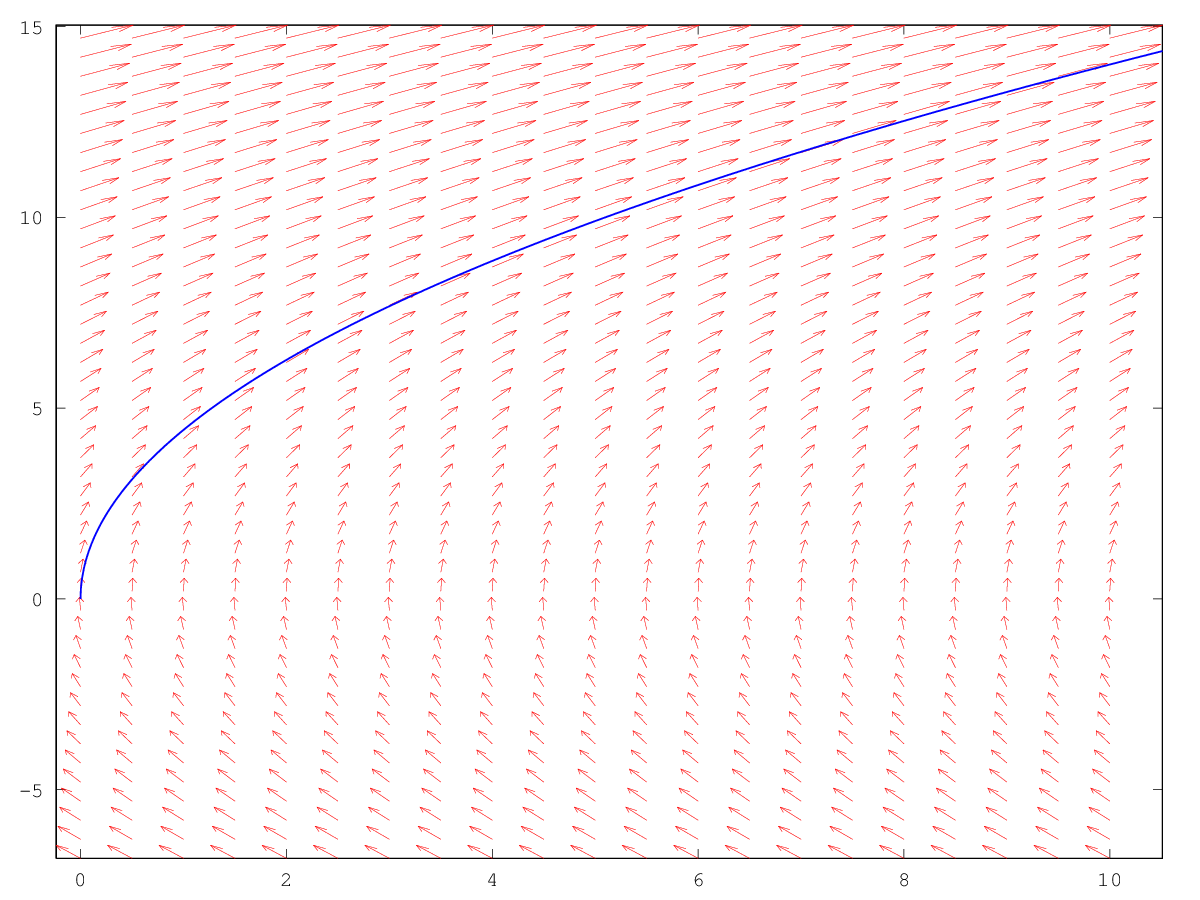
\includegraphics[width=\textwidth]{a_NoDampening}
		\end{figure}
		\item v(t) \begin{figure}[H]
			\caption{Graph of v(t) against t}
			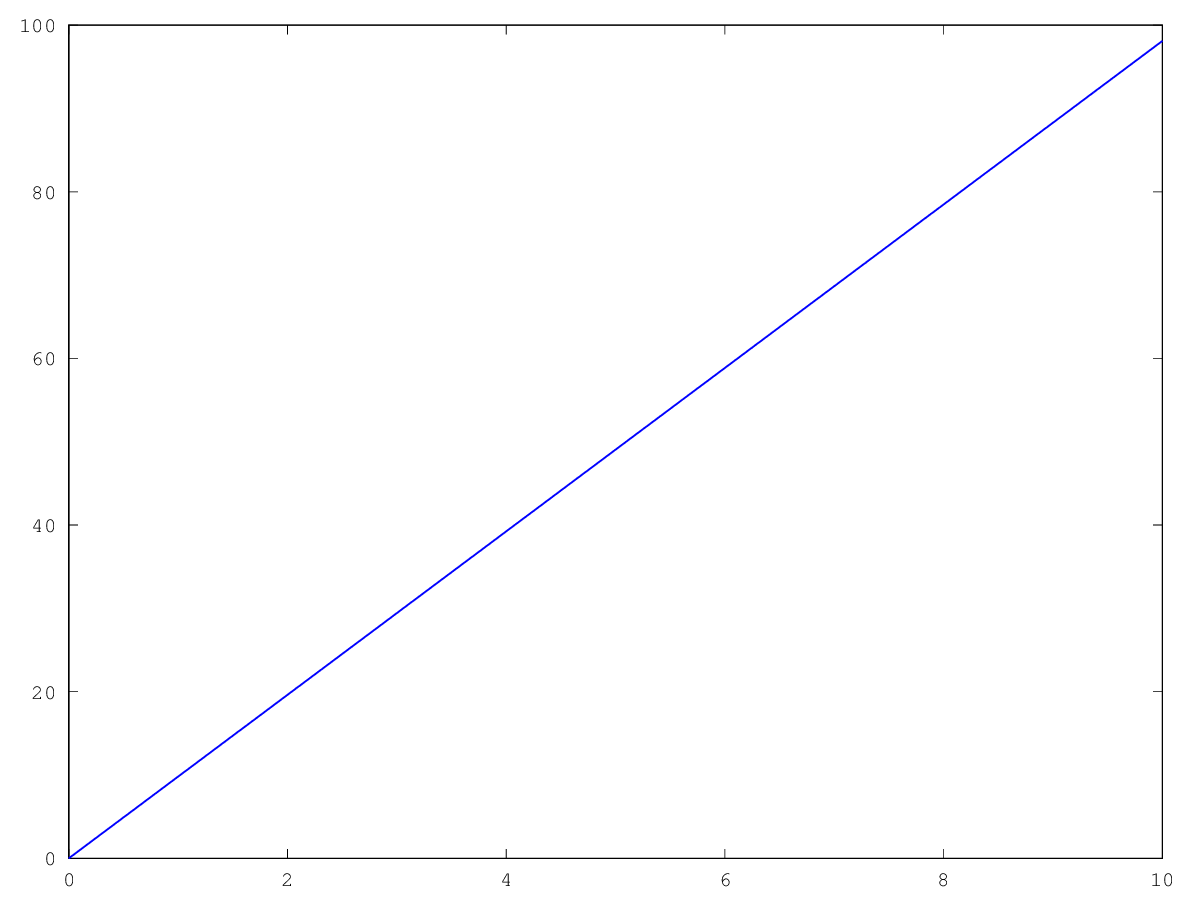
\includegraphics[width=\textwidth]{a_v}
		\end{figure}
		\item x(t) \begin{figure}[H]
			\caption{Graph of x(t) against t}
			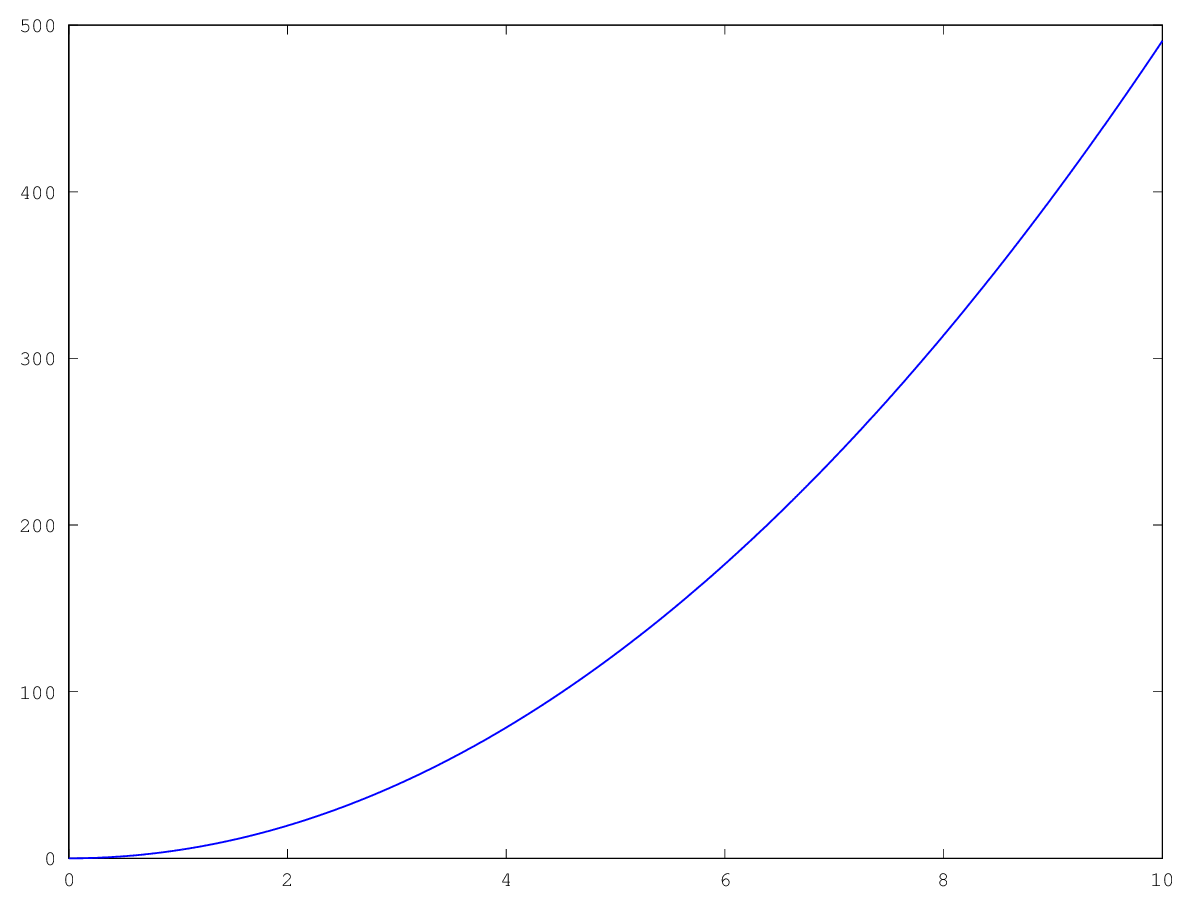
\includegraphics[width=\textwidth]{a_x}
		\end{figure}
	\end{enumerate}
	We can see that there is v and x increase at an increasing rate until a = g at which point a steady state of sorts is achieved.
	
	\item For the steady state solution where $\ddot{x}=0$, we simply start from where $\dot{x}=\sqrt{g} (\therefore \ddot{x}=0)$, at which point we get the following plot:
	\begin{enumerate}[label=(\roman*)]	
		\item Phase Space \begin{figure}[H]
			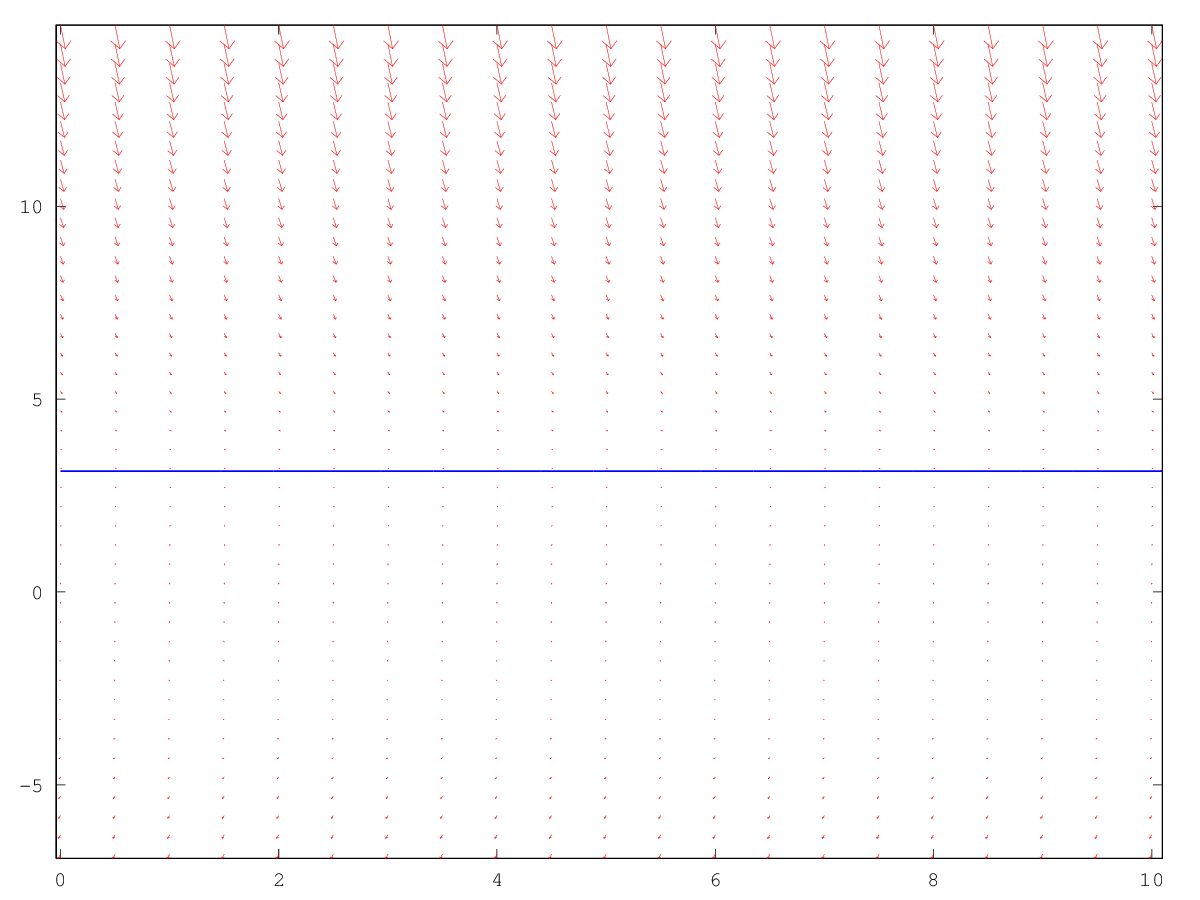
\includegraphics[width=\textwidth]{b_SteadyState}
		\end{figure}
		\item v(t) \begin{figure}[H]
			\caption{Graph of v(t) against t}
			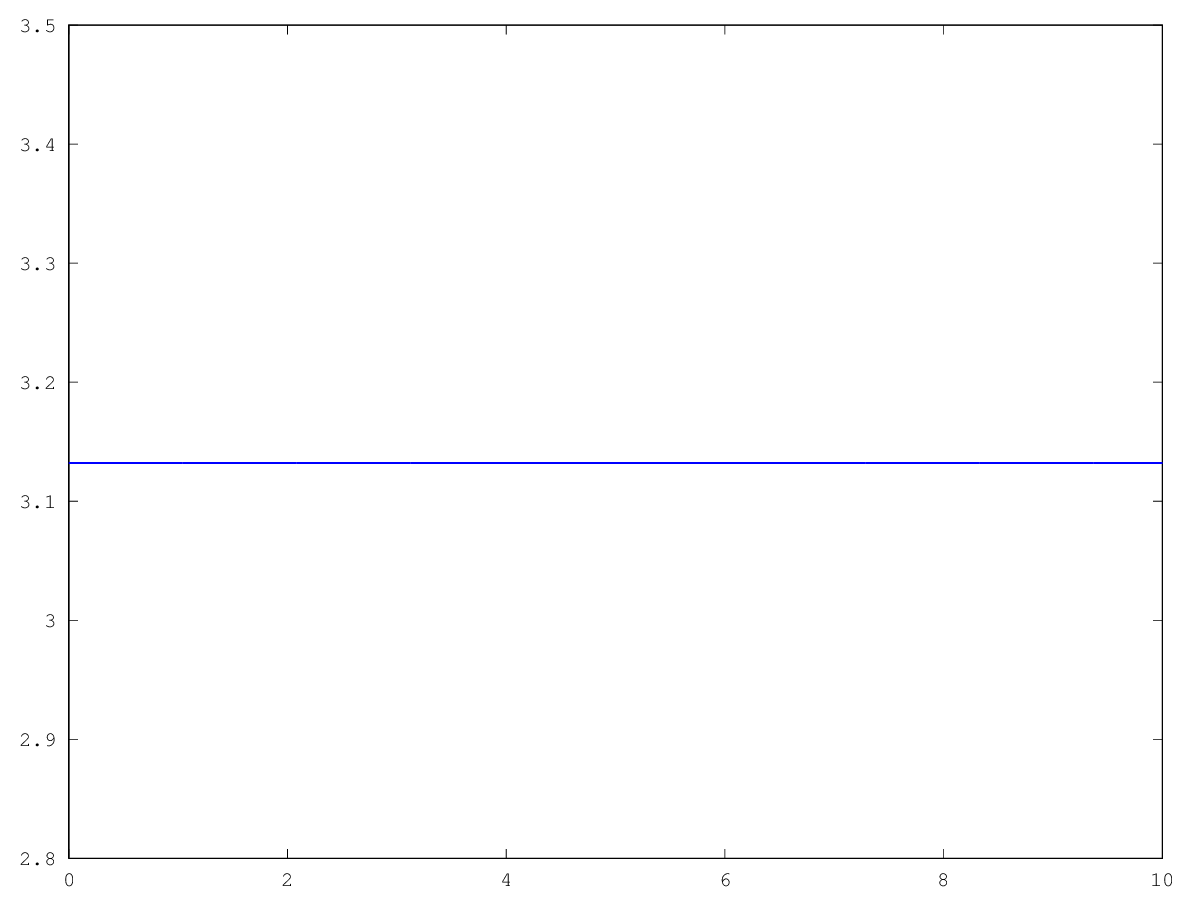
\includegraphics[width=\textwidth]{b_v}
		\end{figure}
		\item x(t) \begin{figure}[H]
			\caption{Graph of x(t) against t}
			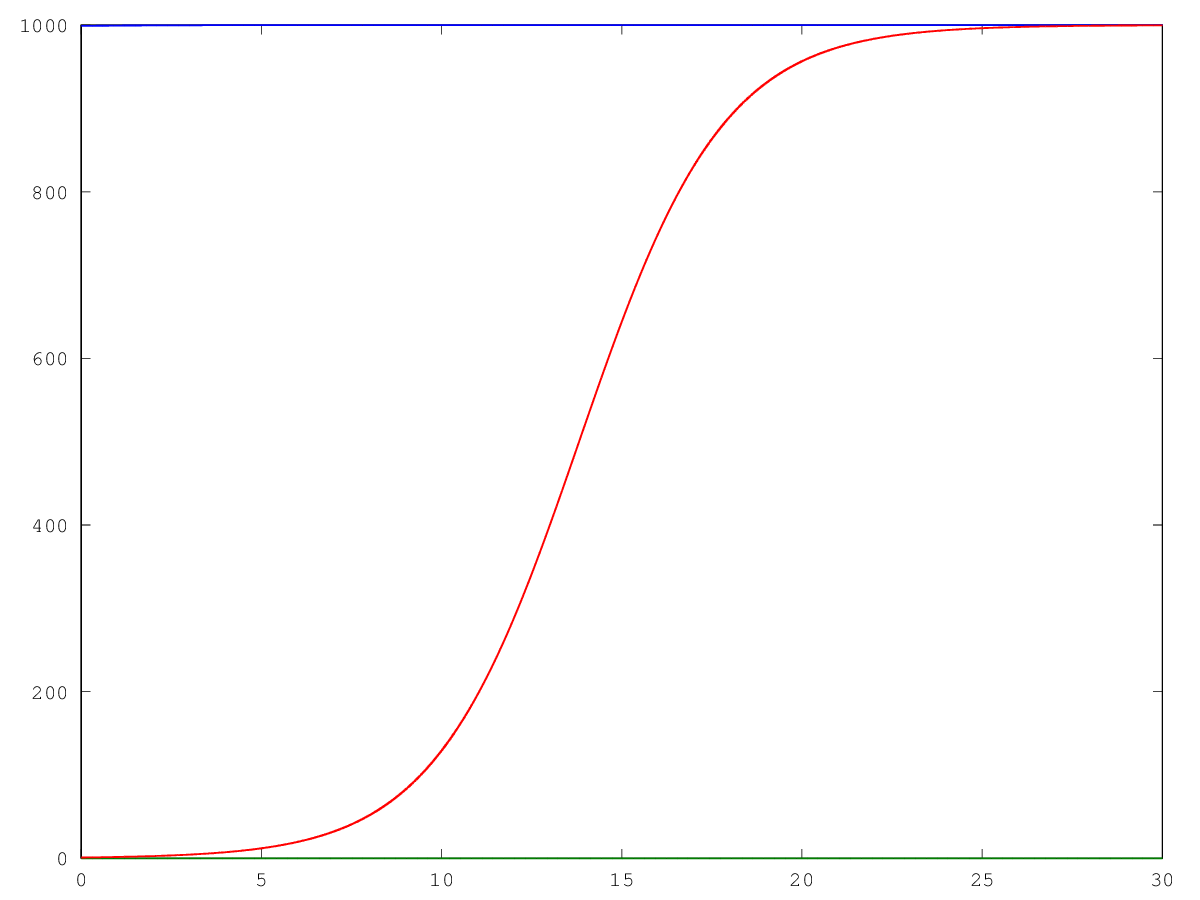
\includegraphics[width=\textwidth]{b_x}
		\end{figure}
	\end{enumerate}
	As expected, x is steadily increasing, v is constant and steady state is achieved.
	
	\item Now the full solution, with x=0, v=0:
	\begin{enumerate}[label=(\roman*)]	
		\item Phase Space \begin{figure}[H]
			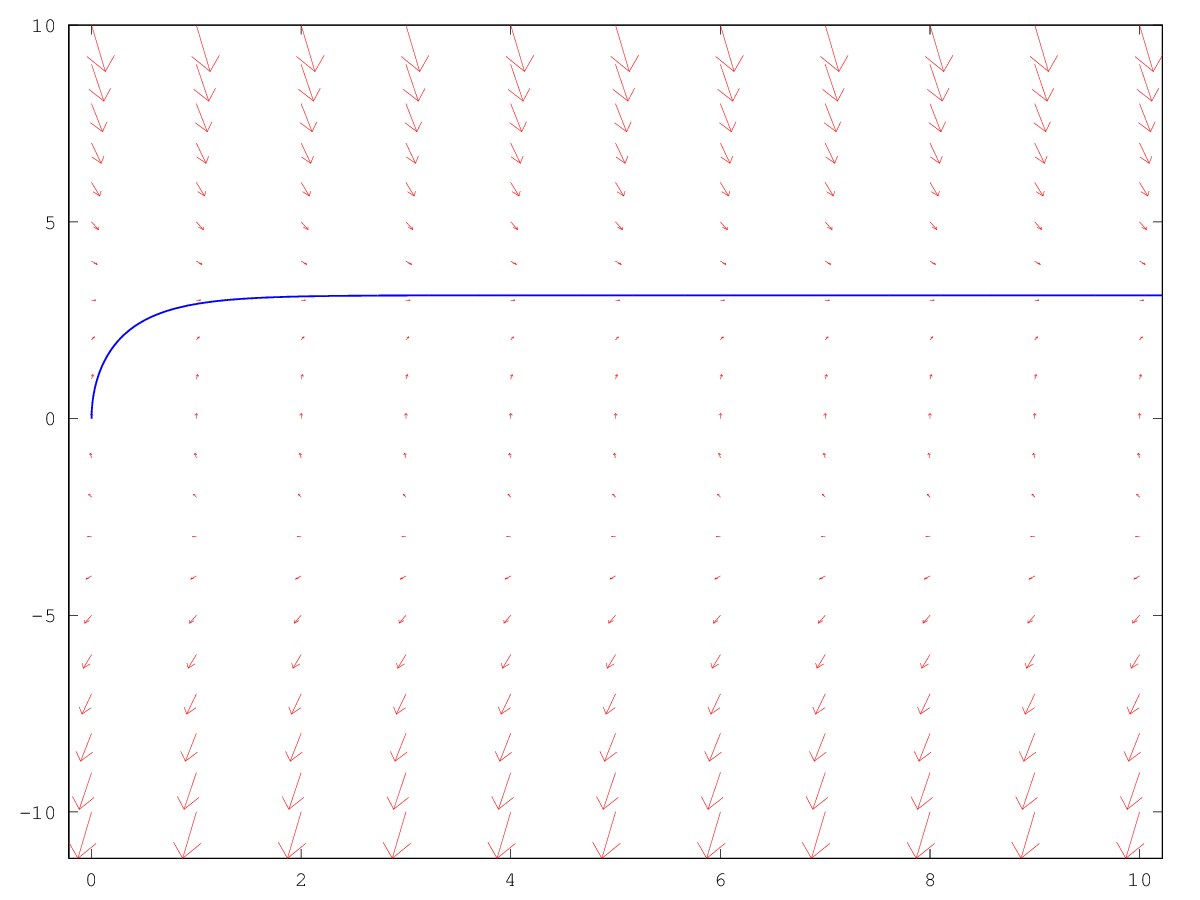
\includegraphics[width=\textwidth]{c_Full}
		\end{figure}
		\item v(t) \begin{figure}[H]
			\caption{Graph of v(t) against t}
			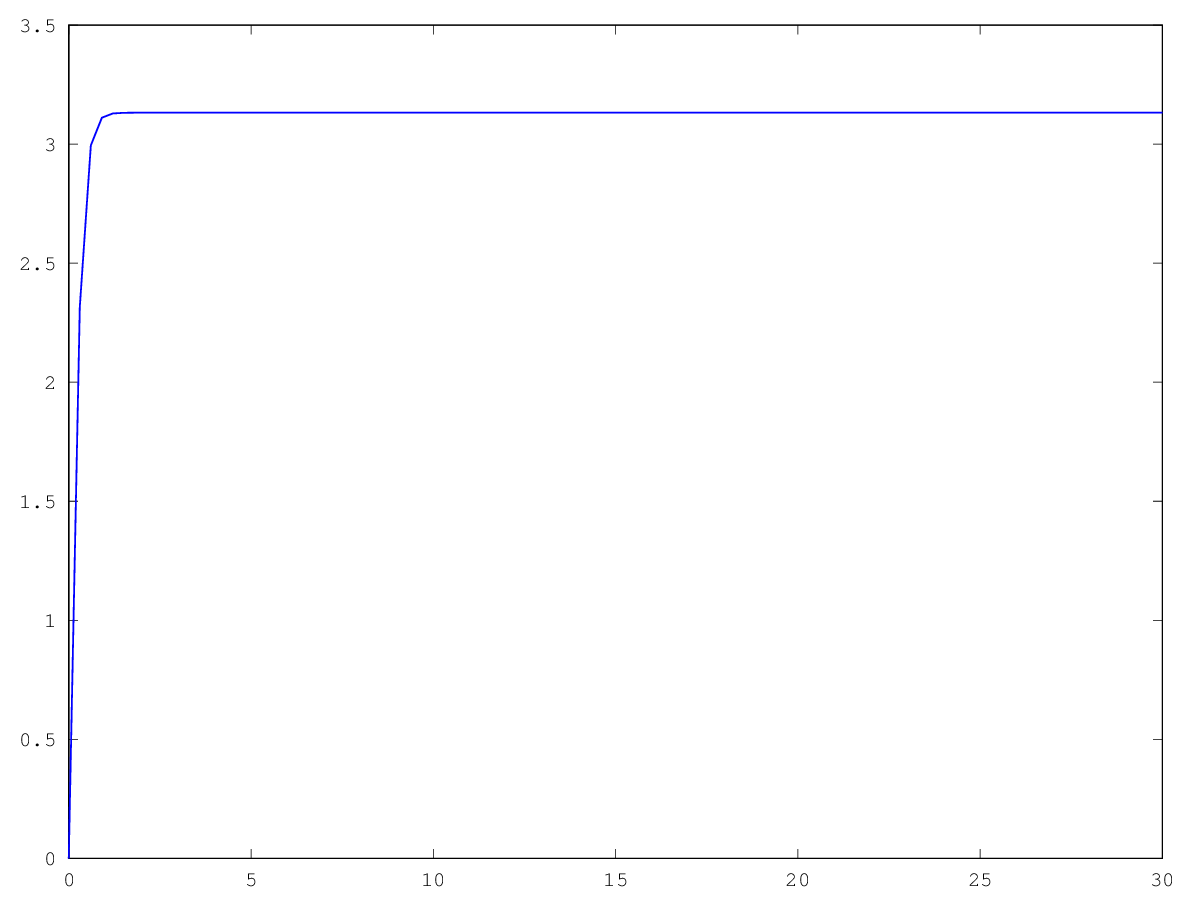
\includegraphics[width=\textwidth]{c_v}
		\end{figure}
		\item x(t) \begin{figure}[H]
			\caption{Graph of x(t) against t}
			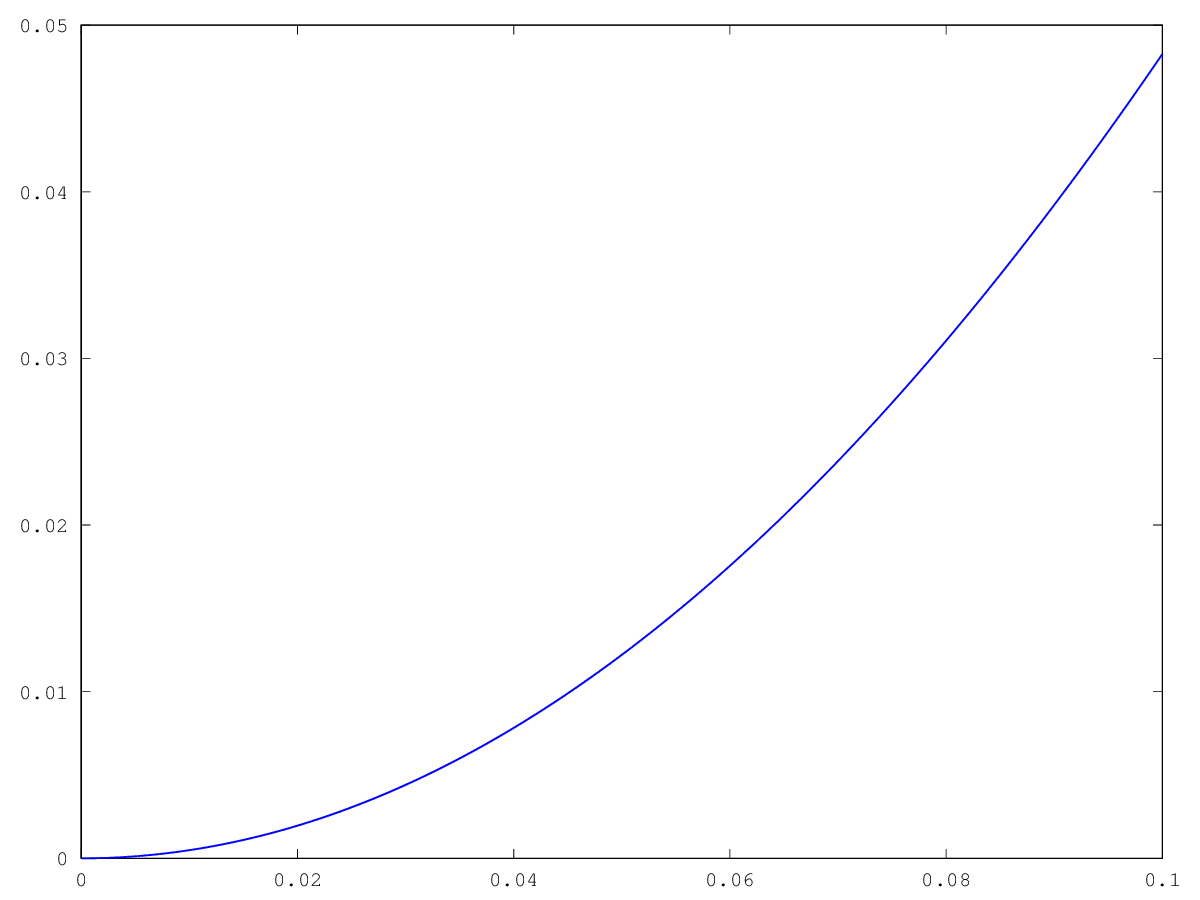
\includegraphics[width=\textwidth]{c_x}
		\end{figure}
	\end{enumerate}
	
	And we can see how the steady state solution is achieved from the origin. The graphs against time are very similar to the sketches we had drawn before.
	
	
	
    \end{enumerate}
	
 
 \end{enumerate} 
 
 \item .3 :
 	For the infinite collection of identical resistors, we can begin with the smallest unit that we can assume exists somewhere inside this infinity:
\begin{figure}[h!]
  \begin{center}
    \begin{circuitikz}
      \draw (0,2)
      to[R=$R_1$] (2,2) % The resistor
      to[short] (2,4);
      \draw (2,2)
      to[short] (2,0);
      \draw (2,0)
      to[R=$R_1$] (4,0) % The resistor
      to[R=$R_1$] (6,0) % The resistor
      to[short] (6,4)
      to[R=$R_1$] (4,4) % The resistor
      to[R=$R_1$] (2,4) % The resisto;
      to[short] (2,4);
      \draw (6,2)
      to[R=$R_1$] (8,2);
    \end{circuitikz}
    \caption{Basic Unit}
  \end{center}
\end{figure}
 
 	The Resistance of this unit is $\frac{2x}{2}+2x$, and we can imagine that each additional level of hierarchy would add add 2x and divide by two, and three levels out we get:
	\[ R = \frac{\frac{\frac{2x}{2}+2x}{2}+2x}{2} \] 
	Combining these transformations, we we can get the following:
	\[ R = 1 + \sum\limits_{i=1}^\infty 2^{-i} = 2 K\Omega \]
	
\end{enumerate}

\end{document}